\newpage
%==========================================================
%--- What programs are and how they are written in our tool
%==========================================================
\section{System Model}
In this section, we first describe our system model including the
notions of distributed applications and replicated data objects,
behavioral properties of eventually consistent data stores and consistency guarantees
over operations. Later, we will formally introduce our specification
language, which helps developers to \emph{specify} their desired consistency
levels. 
%--- The intro the programming model and anomalies
%
\subsection{Replicated Data Stores}
\label{subsec:repl_types}
A data store in our system model, is a collection of \emph{replicas},
each of which stores an instance of a replicated \emph{data object}.
The objects,
which are defined by application developers, contain a \emph{state} that
can be read or modified by application \emph{operations}.
Operations can send requests to replicas to read the current state of the object, or
update it, by producing an \emph{update effect}. 
Effects are then propagated and are guaranteed to reach all replicas
eventually, where they similarly modify the objects' state,
by using an \emph{apply} function, defiened by the developers.

Clients interact
with the store by invoking operations on objects, where a \emph{session} is
the sequence of operations invoked by a particular client. Consequently,
operations
(and the update effects of them) can be uniquely identified, by
their invoking \emph{session id} and their \emph{sequence number} in
that particular session. The data store is typically accessed by a large
number of clients concurrently and consequently, and load balancing
regulations of the store, might cause operations to be routed to different replicas,
even if they are from the same session.

Figure \ref{fig:comment_app}(left) shows how such a  







% one paragraph explaining the given code


% one paragraph exaplining an RMW anomaly and explaining how users can
% just declare what they want



\begin{figure}[t]
        \centering
	\begin{subfigure}[b]{0.489\textwidth}
	\begin{lstlisting}
type Effect = String 
type State =  String 

read :: State -> (String,Maybe Effect)
read s = (s,Nothing)

write :: String -> ((),Maybe Effect)
write comment = ((),comment)

apply :: State -> Effect -> State 
apply s eff = in s ++ " - " ++ comment
	\end{lstlisting}
	\caption{A simple implementation}
	\label{subfig:comment_code}
	\end{subfigure}
	\hfill
	\begin{subfigure}[b]{0.475\textwidth}
	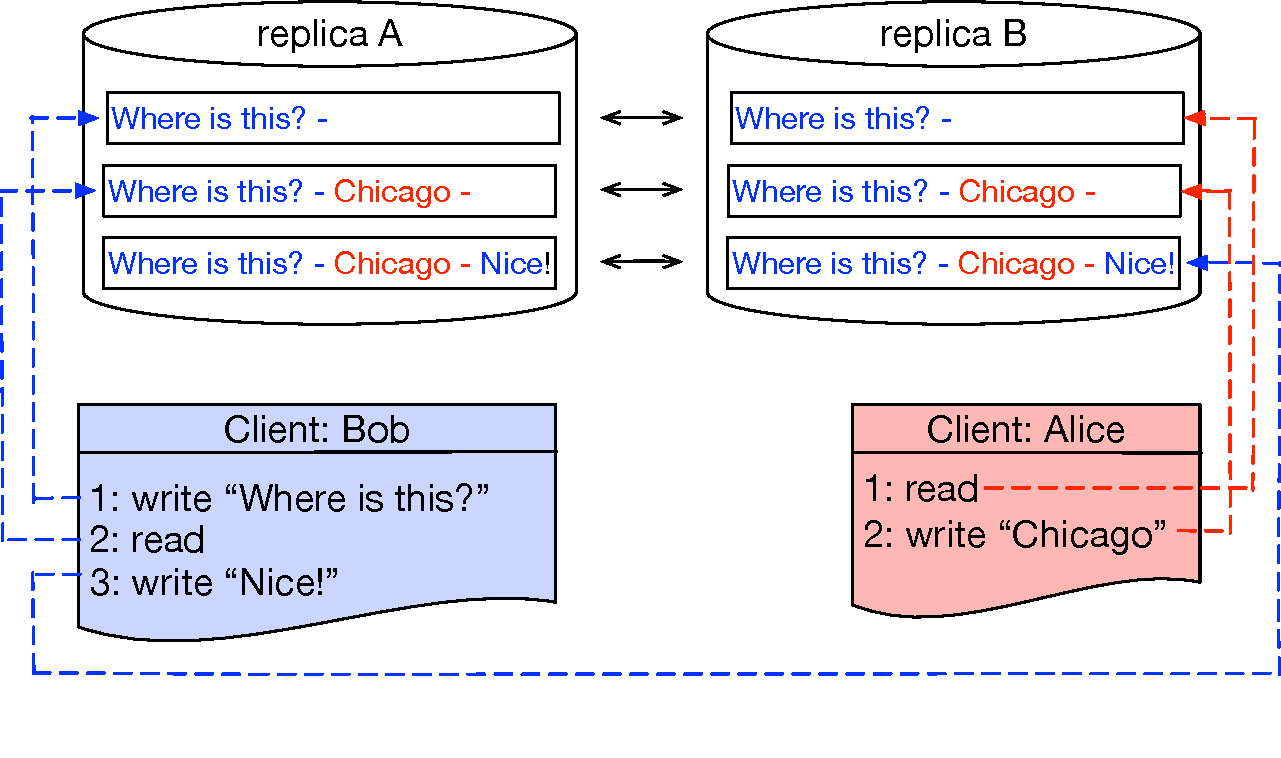
\includegraphics[scale=0.282]{Figures/comment_application.pdf}
	\caption{Example execution}
	\label{subfig:comment_example}
	\end{subfigure} 
\\ \hrulefill
\caption{A distributed application for comment section
management}
\label{fig:comment_app}
\end{figure}





\newpage
%
%--- The introduction of the spec language 
%
\subsection{Specification Language}
\label{subsec:spec_lang}












%==========================================================
\newpage














\begin{comment}
Following is the formal syntax of specification language in our system:
\begin{figure}[t]
\begin{subfigure}{0.41\textwidth}
\centering
  \begin{fmathpar}
  \begin{array}{lclcl}
		\rel & \in & \texttt{rel.seed} & \coloneqq & \visZ \ALT
		\soZ \ALT \rel \cup \rel \\
               \Rel & \in & \texttt{relation} & \coloneqq &  \rel
	       \ALT \Rel;\rel  \ALT \nullR  \\
	     \pi & \in & \texttt{prop} & \coloneqq & \forall a.
      ~a \xrightarrow{R} \hat{\eff} ~\Rightarrow~ a \xrightarrow{\visZ}
      \hat{\eff}\\
		\psi & \in & \texttt{spec} & \coloneqq & \pi \ALT \pi \conj \pi
  \end{array}
  \end{fmathpar}
\subcaption{ syntax of contracts}
\label{fig:ctrt_syntax}
\end{subfigure}
\hfill \vline \hfill
\begin{subfigure}{0.49\textwidth}
\centering
\begin{scriptsize}
\begin{tabular}{|l | c |} 
\hline
 { \texttt Guarantee} & {\texttt Contract} \\ [0.5ex] 
\hline 
\textsc{Read My Writes} & $\forall a. a ~  ~\xrightarrow{\soZ}  ~ ~
\hat{\eta} \Rightarrow a \xrightarrow{\visZ} \hat{\eta} $ \\ 
\textsc{Monotonic Writes} & $\forall a. a \xrightarrow{\soZ;\visZ}
\hat{\eta} \Rightarrow a \xrightarrow{\visZ} \hat{\eta} $ \\ 
\textsc{Monotonic Reads} & $\forall a. a \xrightarrow{\visZ;\soZ}
\hat{\eta} \Rightarrow a \xrightarrow{\visZ} \hat{\eta} $ \\ 
\textsc{Transitive Visibility} & $\forall a. a \xrightarrow{\visZ;\visZ}
\hat{\eta} \Rightarrow a \xrightarrow{\visZ} \hat{\eta} $ \\ 

\hline
\end{tabular}
\end{scriptsize}
\subcaption{examples 
%({\bf R}ead {\bf M}y {\bf W}rites, {\bf M}onotonic
%{\bf W}rites and
%{\bf M}onotonic {\bf R}eads)
}
\label{fig:ctrt_example}
\end{subfigure}
\caption{\tool Specification Language}
\end{figure}

\\ The language is general enough to cover all  the known consistency
levels in the context:
\begin{figure}[h]
  \begin{smathpar}
  \begin{array}{ll}
		\texttt{ Read My Write (RMW): }  & \forall(a,b). a \xrightarrow{so} b ~\Rightarrow~ a \xrightarrow{\visZ} b\\
		\texttt{ Monotonic Reads (MR): }  & \forall(a,b). a \xrightarrow{so;vis} b ~\Rightarrow~ a \xrightarrow{\visZ} b\\
		\texttt{ Monotonic Writes (MW): }  & \forall(a,b). a \xrightarrow{vis;so} b ~\Rightarrow~ a \xrightarrow{\visZ} b\\
		\texttt{ Writes Follow Reads (WFR): }  & \forall(a,b). [a \xrightarrow{vis;vis} b ~\Rightarrow~ a \xrightarrow{\visZ} b] \wedge  
		[a \xrightarrow{vis;so;vis} b ~\Rightarrow~ a \xrightarrow{\visZ} b]\\


  \end{array}
  \end{smathpar}
\caption{Well-known consistency requirements, written in our specification language}
\label{fig:ctrt}
\end{figure}

\\ Specifications written in our language, can be visualized by simple
graphs. For example, \texttt{(MR)} guarantee from the above figure can
be represented as:
\begin{figure}[h]
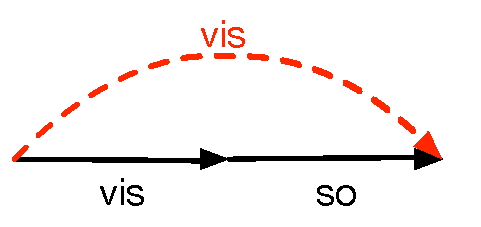
\includegraphics[scale=0.6]{../Figures/MR.pdf}
\caption{A simple way of showing contracts}
\label{fig:ctrt}
\end{figure}


\end{comment}
